\chapter{Integrability in classical mechanics}
\section{Hamiltonian Formalism}
Motion of a system with $n$ degrees of freedom described by trajectory in $2$ dimensional phase space $\mathcal{M}$ (manifold) with \textbf{local} coordinates $(p_j, q_j), j=1,\dots, n$.

\paragraph{Dynamical variables} are some function $f: \mathcal{M}\times \R \rightarrow \R, f=f(p, q, t)$.

\paragraph{Poisson brackets}
\begin{equation}
	\left\{f, g  \right\} := \sum_{i=1}^{k} \pdv{f}{q_k} \pdv{g}{p_k} - \pdv{f}{p_k}\pdv{g}{q_k}
\end{equation}
with the properties
\begin{align*}
	\pb{f}{g} &= - \pb{f}{g}  \\
	\pb{f}{\pb{g}{h}} &+ \pb{g}{\pb{h}{f}} + \pb{h}{\pb{f}{g}}  = 0
	\label{eq:}
\end{align*}
and the canonical ``commutation'' relation
\begin{equation*}
	\pb{p_j}{p_k} 	 = \pb{q_j}{q_k}  = 0, \quad \pb{p_j}{q_k}  = \delta_{jk}
\end{equation*}

Given a Hamiltonian $H = H(p, q, t)$, the dynamics of a dynamical variable is determined by 
\begin{equation*}
	\dv{f}{t} = \pdv{f}{t} + \pb{f}{H}	
\end{equation*}
for any $f = f(p, q)$.

Setting $f=p_j$ or $f=q_j$ yields the Hamilton's equation of motion
\begin{equation}
	\dot{p}_j = - \pdv{H}{q_j}, \quad \dot{q}_j = \pdv{H}{p_j}
	\label{math:ham-eom}
\end{equation}
The system \eqref{math:ham-eom} of $2n$ ordinary differential equations (ODEs) is deterministic, meaning the $(p_j(t), q_j(t))$ are uniquely determined by $2n$ initial conditions.

\begin{definition}
	A function $f= f(p_j, q_j, t)$ which $\dot{f} = 0$, when equation of motion \eqref{math:ham-eom} hold, is called	a \textbf{first integral}, a \textbf{constant of motion}, or a \textbf{conserved charge}.
\end{definition}
Equivalently, $f(p(t), q(t), t) = \text{const}$, if $p(t)$ and $q(t)$ satisfy \eqref{math:ham-eom}.

Hamilton's equations will be solvable, if there are ``sufficiently'' many constants of motion.

\begin{example}
	System with one degree of freedom with $\M = \R^2$ and Hamiltonian $H = \frac{1}{2} p^2 + V(q)$. The Hamilton's equations are
	\begin{equation*}
		\dot{q} = p, \quad \dot{p} = - \pdv{V}{q}	.
	\end{equation*}
	The Hamiltonian $H$ is a first integral	 ($\dv{H} = 0$). Thus,
	\begin{align*}
		\frac{1}{2} p^2 &+ V(q) = E = \text{const} , \\
		\dot{q} &= p, p = \pm \sqrt{2(E-V(q))} , \\
		\Rightarrow t &= \pm \int \frac{\dd{q}}{\sqrt{2(E-V(q))}}
	\end{align*}
	Explicit solution could be found if the integral can be performed and the relation $t=t(q)$ can be inverted to get $q(t)$. These two steps are not always possible, but still it is called \textbf{integrable}.
\end{example}

One can also look at the systems \textbf{geometrically}. First integrals defines $f(p, q)=\text{const.}$ in $\M$. Two hypersurfaces corresponding to two first integrals generically intersect in surface of dimension $2$ in $\M$. In general, trajectory lies on a surface of dimension $(2n-L)$ with $L$ the number of independent first integrals. If $L=2n-1$, this ``surface'' is a curve, i.e. a solution to Hamilton's equations.

The questions now is how to find first integrals? If two first integrals are given, their Poisson bracket is another first integral. Noether's theorem gives first integrals (translations, rotations and so on). Energy is always a first integral in Hamilton formalism.

\section{Integrability and action-angle variables}
\begin{definition}
	Consider a Hamiltonian system with $2n$ dimensional phase space $\M$. We call this system (completely) Louville integrable, if $n$ functions $f_1, \dots, f_n: \M \rightarrow \R$ exists such that
	\begin{itemize}
		\item $\pb{f_j}{f_k} = 0, j, k = 1, \dots, n$
		\item $\pb{H}{f_j} = 0, j=1, \dots, n$
		\item The functions $f_1, \dots, f_n$ are independent, i.e. the $\vec{\nabla} f_j$ are linearly independent vectors on a tangent space to any point in $\M$.
	\end{itemize}
\end{definition}
If condition $(1)$ is satisfied, the $f_j$ are in \textbf{involution}. Integrability in the above sense leads to solvability of equation of motion.

\paragraph{Coordinate transformations}
What freedom is there in Hamiltonian structure?

\begin{definition}
	A transformation $Q_k = Q_k(p, q), P_k = P_k(p, q)$ is canonical, if it preserves the Poisson brackets
	\begin{equation*}
		\pb{f}{g}_{p, q} = \pb{f}{g}_{P, Q}, \forall f,g: \M \rightarrow \R.
	\end{equation*}
\end{definition}
Canonical transformation preserves Hamilton's equations. In $2n$ dimensional phase space, only $2n$ of the coordinates $p, q, P, Q$ are independent. Given a generating function $S(q, P, t)$ with
\begin{equation*}
	\det(\pdv[2]{S}{q_i}{p_k}) = 0	
\end{equation*}
we can construct a canonical transformation by setting 
\begin{equation}
	p_k = \pdv{S}{q_k}, \quad Q_k = \pdv{S}{P_k}, \quad H = H+ \pdv{S}{t}
\end{equation}
There are other possibilities with
\begin{align*}
	S(q, Q):& \; p = \pdv{S}{q} , P=-\pdv{S}{Q} , \\
	S(p, Q):& \; P = -\pdv{S}{Q}, q = - \pdv{S}{Q}, \\
	S(p, P):& \; q = - \pdv{S}{p}, Q= \pdv{S}{P}
	\label{eq:}
\end{align*}
Can we find canonical transformation that manifests integrability such that $P_k(t) = P_k(0) =\text{const}$ $n$ constant of motion and $Q_k(t) = Q_k(0) + t \pdv{H}{p_k}$ with linear time dependence. To find such a transformation is in general hard. Deciding whether a given $H$ is integrable is still unsolved problem.

\begin{theorem} (Arnold and Liouville)
	Let $(\M, f_1, \dots, f_n)$ be integrable system with a Hamiltonian $H=f_1$ and let	
	\begin{equation*}
		\M_f = \left\{ (p, q) \in \M | f_k (p, q) = c_k = \text{const}, k=1, \dots, n \right\} 	
	\end{equation*}
	be a so-called $n$ dimensional level set of first integral $f_n$.
	\begin{itemize}
		\item if $M_f$ is compact and connected, then it is diffeomorphism to torus $T^n = S^1 \times \cdots \times S^1$.
		\item One introduces (neighborhood of this torus in $M$) the action angle variables 
			\begin{equation*}
				I_1, \dots, I_n, \quad \phi_1, \dots, \phi_n, \quad 0 \leq \phi_n \leq 2\pi	
			\end{equation*}
			such thant the angles $\phi_k$ are coordinates on $M_f$ and the action (variable) $I_k=I_k(f_1, \dots, f_n)$ are first integrals.
		\item The canonical equations of motion \eqref{math:ham-eom} becomes
			\begin{equation}
				\dot{I}_k = 0, \quad \dot{\phi}_k = \omega_k (I_1, \dots, I_n), \quad k =1, \dots,n 
				\label{math:action-angle-eom}
			\end{equation}
			and the integrable system is solved by \textbf{quadratures} (finite number of algebraic equations and integrations of know functions).
	\end{itemize}
\end{theorem}

\paragraph{Proof} (not to prove $(1)$ here). On $(2)$ and $(3)$

Motion takes place on surface of dimension $2n -n = n$
\begin{equation}
	f_1 (p,q) = c_1, \dots, f_n(p, q) = c_n .
	\label{math:arnold-theorem-first-integral}
\end{equation}
From $(1)$, this surface is a torus. Assume $\det(\pdv{f_i}{p_k}) \neq 0$ such that \eqref{math:arnold-theorem-first-integral} can be solved for the momenta $p_i = p_i (q, c)$ with $f_i(q, p(q,c )) = c_i$
\begin{align*}
	\pdv{q_j} & \Rightarrow \pdv{f_i}{q_j} + \sum_{k=0}^{n} \pdv{f_i}{p_k} \pdv{p_k}{q_j} = 0, \\
	 \sum_j \cdot \pdv{f_i}{p_j} &\Rightarrow \sum_j \pdv{f_m}{p_j} \pdv{f_i}{q_j} + \sum_{j, k} \pdv{f_m}{p_j}\pdv{f_i}{p_k} \pdv{p_k}{q_j} = 0, \\
	(mi) - (im) &\Rightarrow \pb{f_i}{f_m} + \sum_{j, k} \left( \pdv{f_m}{p_j} \pdv{f_i}{p_k} \pdv{p_k}{q_j} - \pdv{f_i}{p_j} \pdv{f_m}{p_k} \pdv{p_k}{q_j} \right)  = 0, \\
					&\Rightarrow \sum_{j, k} \pdv{f_i}{p_k} \pdv{f_m}{p_j} \left( \pdv{p_k}{q_j} - \pdv{p_j}{q_k} \right)  = 0, \\
	\left( \pdv{f_i}{p_k} \right) \text{ invertible} &\Rightarrow \pdv{p_k}{q_j} - \pdv{p_j}{q_k} = 0, \\
	\text{Stockes' theorem} &\Rightarrow \oint_{\mathcal{G}} \sum_{j=1}^{n} p_j \dd{q_j} = 0,
\end{align*}
for any closed curve on torus $T^n$ such are contractible to a point. 

On $T^n$ there are $n$ closed curves that cannot be contracted to a point, such that the corresponding integrals do not vanish.

\begin{definition}
\textbf{action variable}

\begin{equation}
	I_k := \frac{1}{2\pi} \oint_{\Gamma_k} \sum_{i=1}^{n} p_j \dd{q_j}, \quad k = 1, \dots, n
	\label{math:action-variable-def}
\end{equation}
where the curve $\Gamma_k$ is the $k$-th basic cycle on the torus $T^n$
\begin{equation*}
\Gamma_k = \left\{ (\tilde{\phi}_1, \dots \tilde{\phi}_n) \in T^n; 0 \leq \tilde{\phi}_k \leq 2\pi, \tilde{\phi}_j = \text{const, for} j\neq k  \right\}.
\end{equation*}
\todo{Why is this integral not zero? Compactness?}

\end{definition}
$\tilde{\phi}_k$ denotes some coordinates on $T^n$. This is non-trivial, in practice it is not clear how to describe a torus explicitly. Arnold-Liouville theorem has character of existence theorem. \todo{why is it non-trivial? In 2d case, they can be parametrised easily.}

Stockes theorem implies the action \eqref{math:action-variable-def} are independent of choice of $\Gamma_k$. The action \eqref{math:action-variable-def} are first integrals since $\oint p(q, c) \dd{q}$ only depend on $c_k = f_k$ and $f_k$'s are first integrals.

We have all the action variable in involution, since
\begin{align*}
	\pb{I_i}{I_j} &= \sum_{r, s, k} \left( \pdv{I_i}{f_r} \pdv{f_r}{q_k} \pdv{I_j}{f_s} \pdv{f_s}{p_k} - \pdv{I_i}{f_r} \pdv{f_r}{p_k} \pdv{I_j}{f_s} \pdv{f_s}{q_k} \right),  \\
					  &= \sum_{r,s} \pdv{I_j}{f_r} \pdv{I_j}{f_s} \pb{f_r}{f_s}, \\
					  &=0.
	\label{eq:}
\end{align*}
In particular $\pb{I_k}{H}=0$. The torus $\mathcal{M}_f$ can be equivalently defined ny 
\begin{equation*}
	I_1 = \tilde{c}_c, 	\dots, I_n = \tilde{c}_n
\end{equation*}

One may ask why is $I_k$ (as coordinate) better than $f_k$. If one defines $I_k = f_k$, the transformation $(p, q) \rightarrow (I, \phi)$ would not be canonical. 

Canonical \textbf{angle} coordinates $\phi_k$, which is the canonically conjugate to the actions via the generating functions
\begin{equation}
	S(q, I) = \int_{q_0}^{q} \sum_j p_j \dd{q_j}
\end{equation}
with $q_0$ some point on the torus. Modifying $q_0$ just adds a constant to $S$. The angle coordinates are
\begin{equation*}
	\phi_i = \pdv{S}{I_i}.
\end{equation*}
The angles are periodic. Consider two paths $C$ and $C \cup C_k$ (with $C_k = \Gamma_k$ the $k$-th cycle) between $q_0$ and $q$, see figure \ref{fig:torus-angle}.
\begin{figure}[ht]
	\centering
	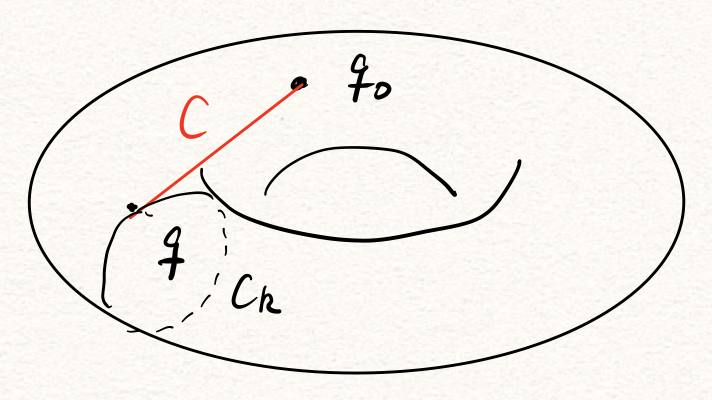
\includegraphics[width=0.5\textwidth]{./figs/torus-angle.jpg}
	\caption{Torus with two paths $C$ and $C\cup C_k$}
	\label{fig:torus-angle}
\end{figure}
Then
\begin{align*}
	S(q, I) &= \int_{C\cup C_k} \sum_j p_j \dd{q_j} \\
			  &= \int_{C} \sum_j p_j \dd{q_j} + \int_{C_k = \Gamma_k} \sum_j p_j \dd{q_j} \\
			  &= S(q, I) + 2\pi I_k \\
	\Rightarrow \phi_k &= \pdv{S}{I_k} = \phi_k + 2\pi
	\label{eq:}
\end{align*}

The transformation
\begin{equation*}
	q = q(\phi, I), \quad p = p(\phi, I)
\end{equation*}
and 
\begin{equation*}
	\phi = \phi(p, q) ,\quad I = I(p, q)
\end{equation*}
are canonical transformations (defined by the generating function $S$) and invertible. The Poisson structures are unchanged
\begin{align*}
	\pb{I_j}{I_k} = 0, \quad \pb{\phi_j}{\phi_k} = 0, \quad \pb{\phi_j}{I_k} = \delta_{jk}
	\label{eq:}
\end{align*}
The dynamics are given by
\begin{align*}
	\dot{\phi}_k = \pb{\phi_k}{\tilde{H}}, \quad \dot{I}_k = \pb{I_k}{\tilde{H}}
\end{align*}
with $\tilde{H} = \tilde{H}(\phi, I) = H(q(\phi, I), p(\phi, I))$. Since $I_k$'s are first integrals, 
\begin{equation*}
	0 = \dot{I}_k = \pdv{\tilde{H}}{\phi_k} ,
\end{equation*}
in other word $\tilde{H} = \tilde{H}(I)$. The derivatives of angle variable
\begin{equation*}
	\dot{\phi}_k = \pdv{\tilde{H}}{I_k} = \omega_k (I)
\end{equation*}
are first integrals as well.

Integration (``integrable'' model) yields
\begin{align}
	\begin{split}
		\phi_k (t) &= \omega_k(I) t + \phi_k (0), \\
		I_k(t) &= I_k(0).
	\end{split}
	\label{math:action-angle-sol}
\end{align}
The system is in a circular motion with constant angular velocity.

\paragraph{Geometric picture}
The phase space of an integrable system  is  foliated into an $n$-parameter ($c_j$) family of invariant tori on which flow is linear with constant frequency $\omega_k$. The trajectory \eqref{math:action-angle-sol} may be closed on the torus or it may cover it densely. For $n=2$, the trajectory is closed if $\omega_1/\omega_2$  is rational and dense otherwise.

\paragraph{Degeneracy}
The periodicity in $\phi$ means that every function $F(p, q)$ of the state of system is periodic in $\phi$. Expand the function in Fourier series, e.g. $n=2$
\begin{align*}
	F &= \sum_{l_1 = -\infty}^{\infty}\sum_{l_2 = -\infty}^{\infty} B_{l_1, l_2} \exp(i (l_1 \phi_1 + l_2\phi_2)), \\
	  &= \sum_{l_1, l_2} B_{l_1, l_2} \exp(it(l_1 \omega_1 + l_2 \omega_2)).
\end{align*}
Every summand is period with frequency $l_1\omega_1 + l_2\omega_2$. Sum of functions is not necessarily periodic. The whole sum is only periodic for rational $\omega_1 / \omega_2$. If $a_j \omega_j = a_k \omega_k$ for $a_{j, k} \in \Z$ for some $j, k$, one speaks of \textbf{degeneracy}. If $a_1\omega_1 = \dots = a_n \omega_n$, the system is \textbf{maximally} degenerate.

\paragraph{Example}
All time-indepedent Hamiltonian systems with $2$ dimensional phase-space are integrable ($H=f_{1=n}$). 

Consider a harmonic oscillator ($n=1$) with the Hamiltonian
\begin{equation*}
	H = \frac{1}{2} (p^2 + \omega^2 q^2)
\end{equation*}
Different choices of energy $c_1 = E$ give foliation of $\M$ by ellipses
\begin{equation*}
	\frac{1}{2} \left( p^2 + \omega^2 q^2 \right) 	 = E
\end{equation*}
with two axes $a = \sqrt{2E}$ and $b = \frac{\sqrt{2E}}{\omega}$ and surface $ab\pi$. For fixed $E$, take $\Gamma = \M_H$
\begin{equation*}
	I = \frac{1}{2\pi} \oint d\dd{q} \stackrel{\text{Stockes'}}{=} \frac{1}{2\pi} \int_{S} \dd{p} \dd{q} = \frac{E}{\omega}
\end{equation*}
The Hamiltonian in the new variable $\tilde{H} = \omega I$ and $\dot{\phi} = \pdv{\tilde{H}}{I} = \omega$, $\phi = \omega t + \phi_0$. 

To obtain the transformation $(p, q) \rightarrow (I, \phi)$, first the action variable is
\begin{equation*}
	I(p, q) = \frac{1}{\omega}H(p, q) = \frac{1}{2} \left( \frac{1}{\omega} p^2 + \omega q^2 \right) .
\end{equation*}
The generating function is
\begin{equation*}
	S(q, I ) = \int_{q_0}^{q} p \dd{\tilde{q}} = \pm \int_{q_0}^{q} \sqrt{2 I \omega - \omega^2 \tilde{q}} \dd{\tilde{q}}
\end{equation*}
and the angle variable
\begin{equation*}
	\phi = \pdv{S}{I} = \int \frac{\omega\ \dd{\tilde{q}}}{\sqrt{2I\omega - \omega^2 \tilde{q}^2}} = \arcsin(q \sqrt{\frac{\omega}{2I}}) - \phi_0.
\end{equation*}
Thus
\begin{align*}
	q &= \sqrt{\frac{2 E}{\omega}} \sin(\omega t + \phi_0) \\
	p &= \pdv{H}{p} = \dot{q} = \sqrt{2E} \cos(\omega t + \phi_0)
\end{align*}
